\documentclass[14pt]{beamer}
\usepackage{fontspec}
\usepackage{color}
\usepackage{minted}

%% These fonts are non-free.
%% Comment out the lines if you don't have them.
\setmainfont{Equity Text A}
\setsansfont{Concourse T3}
\setmonofont{Triplicate T4}

\definecolor{bgcolor}{RGB}{20,25,28}
\setbeamercolor{background canvas}{bg=bgcolor}
\setbeamercolor{normal text}{fg=white}
\setbeamercolor{itemize item}{fg=white}
\setbeamertemplate{itemize items}[circle]
\usemintedstyle{monokai}

\renewcommand{\theFancyVerbLine}{\color{darkgray}\large \oldstylenums{\arabic{FancyVerbLine}}}
\newcommand{\toptitle}[1]{
  {\huge #1} \\
  \vspace{0.2cm}
}
\renewcommand{\subtitle}[1]{
  {\large #1} \\
  \vspace{0.2cm}
}

\begin{document}
\begin{frame}
  \begin{center}
    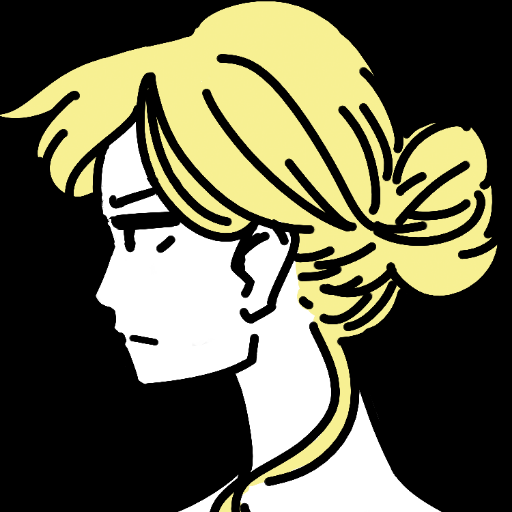
\includegraphics[height=4cm]{avatar.png}\\
    \vspace{0.2cm}
    {\Large Nicolas Hafner} \\
    \vspace{0.2cm}
    {\Huge @Shinmera} \\
    \vspace{0.2cm}
    \url{https://everything.shinmera.com}
  \end{center}
\end{frame}

\end{document}

%%% Local Variables:
%%% mode: latex
%%% TeX-master: t
%%% TeX-engine: luatex
%%% TeX-command-extra-options: "-shell-escape"
%%% End:
